% ----------------------------------------------------------
% Introdução
% ----------------------------------------------------------
\chapter{Introdução}

O crescimento do número de pessoas que vivem sozinhas tem sido descrito como um fenômeno global de caráter epidêmico. Segundo a Universidade de Üsküdar, ``living alone has become an epidemic'' \cite{erdogan2024}. Essa realidade impacta diretamente a saúde e o bem-estar, especialmente entre idosos e indivíduos com necessidades especiais.

Pesquisas publicadas no \textit{European Journal of Public Health} demonstram que indivíduos que vivem sozinhos apresentam maior probabilidade de necessitar hospitalizações de emergência \cite{kandler2017}. De forma complementar, estudos da \textit{Revista Brasileira de Enfermagem} evidenciam que idosos em moradias unipessoais estão mais sujeitos a quedas e fraturas, sobretudo aqueles com doenças cognitivas \cite{perseguino2017}.

No Brasil, dados da PNAD/IBGE revelam que mais de 4,3 milhões de pessoas com mais de 65 anos vivem em moradias unipessoais. Paralelamente, estatísticas do Ministério da Saúde mostram tendência de crescimento nas mortes por acidentes domésticos, influenciadas pelo envelhecimento populacional e pelo aumento de lares unipessoais.

Apesar da gravidade do cenário, observa-se uma lacuna significativa na oferta de soluções acessíveis e não invasivas voltadas ao monitoramento contínuo dessas pessoas. Relatórios do Australian Institute of Family Studies apontam que o isolamento residencial está relacionado a impactos negativos no bem-estar físico e psicológico \cite{aifs2014}.

Diante desse panorama, surge o projeto Linha Vital, que propõe o desenvolvimento de um sistema mobile capaz de monitorar períodos de inatividade, enviar notificações periódicas e acionar automaticamente contatos de confiança e serviços de emergência. A solução busca integrar tecnologia e cuidado de forma equilibrada, promovendo maior autonomia sem comprometer a segurança dos usuários.

\section{Objetivos}

O propósito central do sistema de cuidados e chamadas emergenciais Linha Vital é desenvolver uma solução tecnológica acessível e não invasiva, capaz de monitorar a inatividade de indivíduos que vivem sozinhos e possuem necessidades especiais. A proposta busca oferecer um mecanismo confiável de suporte, acionando automaticamente contatos de confiança e serviços de emergência em situações de risco, de modo a reduzir o tempo de resposta em eventos críticos e aumentar a segurança sem comprometer a autonomia dos usuários.

Para alcançar esse objetivo geral, o projeto contempla um conjunto de metas específicas que orientam sua implementação e funcionamento. Entre elas, destaca-se o desenvolvimento de funcionalidades voltadas ao monitoramento contínuo da inatividade, permitindo a identificação de padrões que indiquem situações atípicas. Além disso, pretende-se implementar mecanismos de envio de notificações periódicas, com o intuito de confirmar o estado de bem-estar do indivíduo e garantir uma interação mínima necessária para validação de sua condição.

Complementarmente, o sistema deve ser capaz de gerar alertas automáticos em casos de ausência de resposta, acionando previamente contatos cadastrados ou serviços de emergência conforme o nível de criticidade identificado. Também se propõe a disponibilização de recursos de acionamento manual, como botões de pânico, bem como funcionalidades voltadas à acessibilidade, assegurando que usuários com diferentes limitações possam utilizar o sistema de forma eficiente.

Por fim, o projeto tem como diretriz oferecer suporte direcionado a idosos e pessoas com necessidades especiais, promovendo maior autonomia no cotidiano sem comprometer sua segurança. Ao integrar tecnologia e cuidado de forma equilibrada, o Linha Vital busca contribuir para a melhoria da qualidade de vida e para a construção de um ambiente doméstico mais seguro e inclusivo.

\section{Problema e Solução Proposta}

O crescimento do número de pessoas que vivem sozinhas tem sido apontado como uma tendência global relevante, descrita em alguns contextos como um fenômeno de caráter epidêmico. Esse cenário envolve, de forma significativa, idosos, pessoas com condições crônicas de saúde e indivíduos em situação de vulnerabilidade emocional, que passam longos períodos sem supervisão direta.

Estudos indicam que viver sozinho está associado a riscos concretos à saúde e à segurança. Pesquisas publicadas no \textit{European Journal of Public Health} demonstram que indivíduos nessa condição apresentam maior probabilidade de hospitalização de emergência \cite{kandler2017}.

De forma complementar, relatórios do Australian Institute of Family Studies apontam que o isolamento residencial está relacionado a impactos negativos no bem-estar físico e psicológico, além de aumentar a exposição a eventos críticos sem assistência imediata \cite{aifs2014}.

Nesse contexto, identifica-se uma lacuna relevante: a ausência de mecanismos acessíveis, contínuos e não invasivos que permitam o acompanhamento indireto do bem-estar desses indivíduos, bem como o acionamento rápido de contatos de confiança em situações de risco.

Como consequência, emergências como quedas, mal súbito ou crises emocionais podem permanecer sem resposta por períodos críticos, elevando significativamente o risco de agravamento clínico ou até mesmo de óbito evitável.

Diante desse cenário, o sistema Linha Vital propõe uma solução baseada em monitoramento inteligente e acionamento automatizado de emergências por meio de um aplicativo mobile. A proposta fundamenta-se na detecção de padrões de ausência de atividade, utilizando esse comportamento como indicador indireto de risco.

O sistema permite o cadastro de contatos de confiança e de emergência, que podem ser acionados automaticamente quando determinadas condições forem atendidas, como períodos prolongados sem resposta. Como mecanismo complementar de segurança, o usuário também pode realizar o acionamento manual por meio de recursos de acessibilidade do próprio dispositivo, garantindo resposta imediata em situações conscientes de risco.

A solução opera em múltiplas camadas de proteção, buscando reduzir o tempo de resposta em emergências e aumentar a segurança sem comprometer a autonomia do usuário: preventiva (monitoramento), reativa automática (inatividade) e reativa manual (acionamento direto).

Dessa forma, o Linha Vital posiciona-se como uma alternativa prática, acessível e centrada no uso doméstico, oferecendo suporte contínuo a indivíduos em situação de vulnerabilidade sem a necessidade de infraestrutura complexa ou monitoramento constante por terceiros.

\section{Justificativa}

Diante das problemáticas relacionadas a indivíduos com necessidades especiais, especialmente a população idosa que reside sozinha, torna-se necessário mensurar a dimensão desse grupo vulnerável.

O Gráfico~\ref{fig_idosos} apresenta a taxa de idosos vivendo sozinhos no Brasil.

\begin{figure}[H]
\caption{\label{fig_idosos}Taxa de idosos vivendo sozinhos.}
\begin{center}
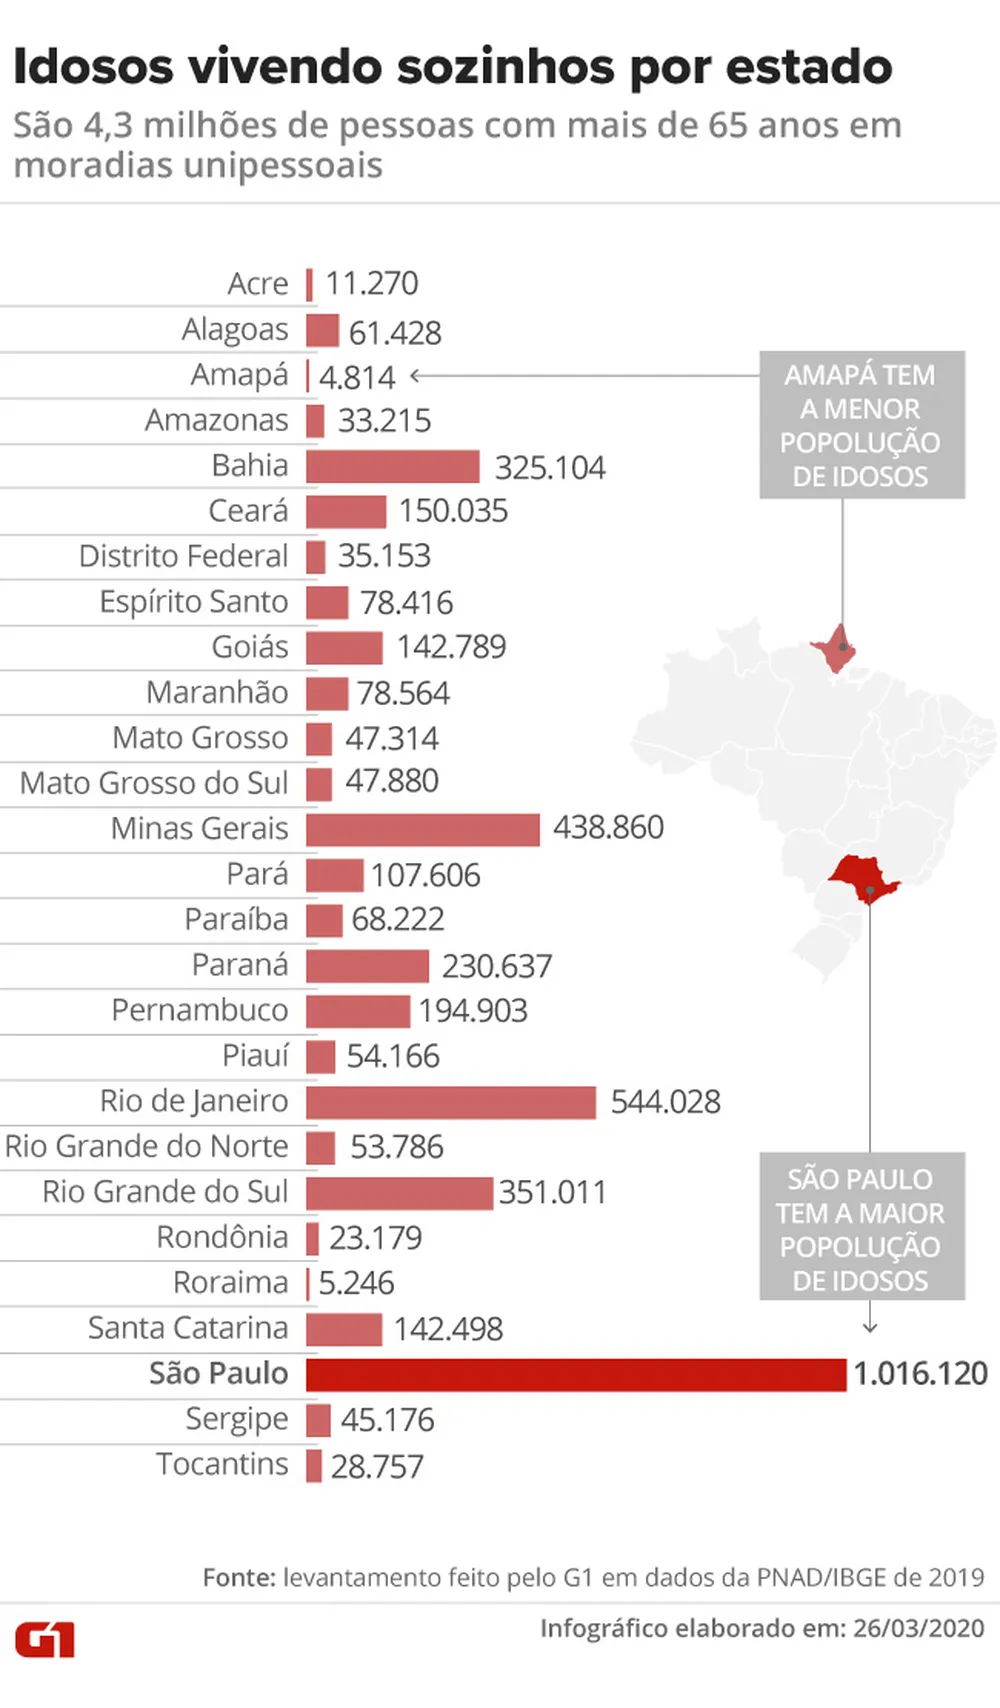
\includegraphics[scale=0.3]{imagens/idosos_sozinhos.png}
\end{center}
\legend{Fonte: PNAD/IBGE via G1 (2020).}
\end{figure}

O número de mortes por acidentes domésticos no Brasil apresenta tendência de crescimento ao longo dos anos. Esse fenômeno sofre influência do aumento da população idosa e do crescimento dos lares unipessoais.

A Figura~\ref{fig_acidentes} apresenta a evolução das mortes por acidentes domésticos no Brasil.

\begin{figure}[H]
\caption{\label{fig_acidentes}Mortes por acidentes domésticos no Brasil.}
\begin{center}
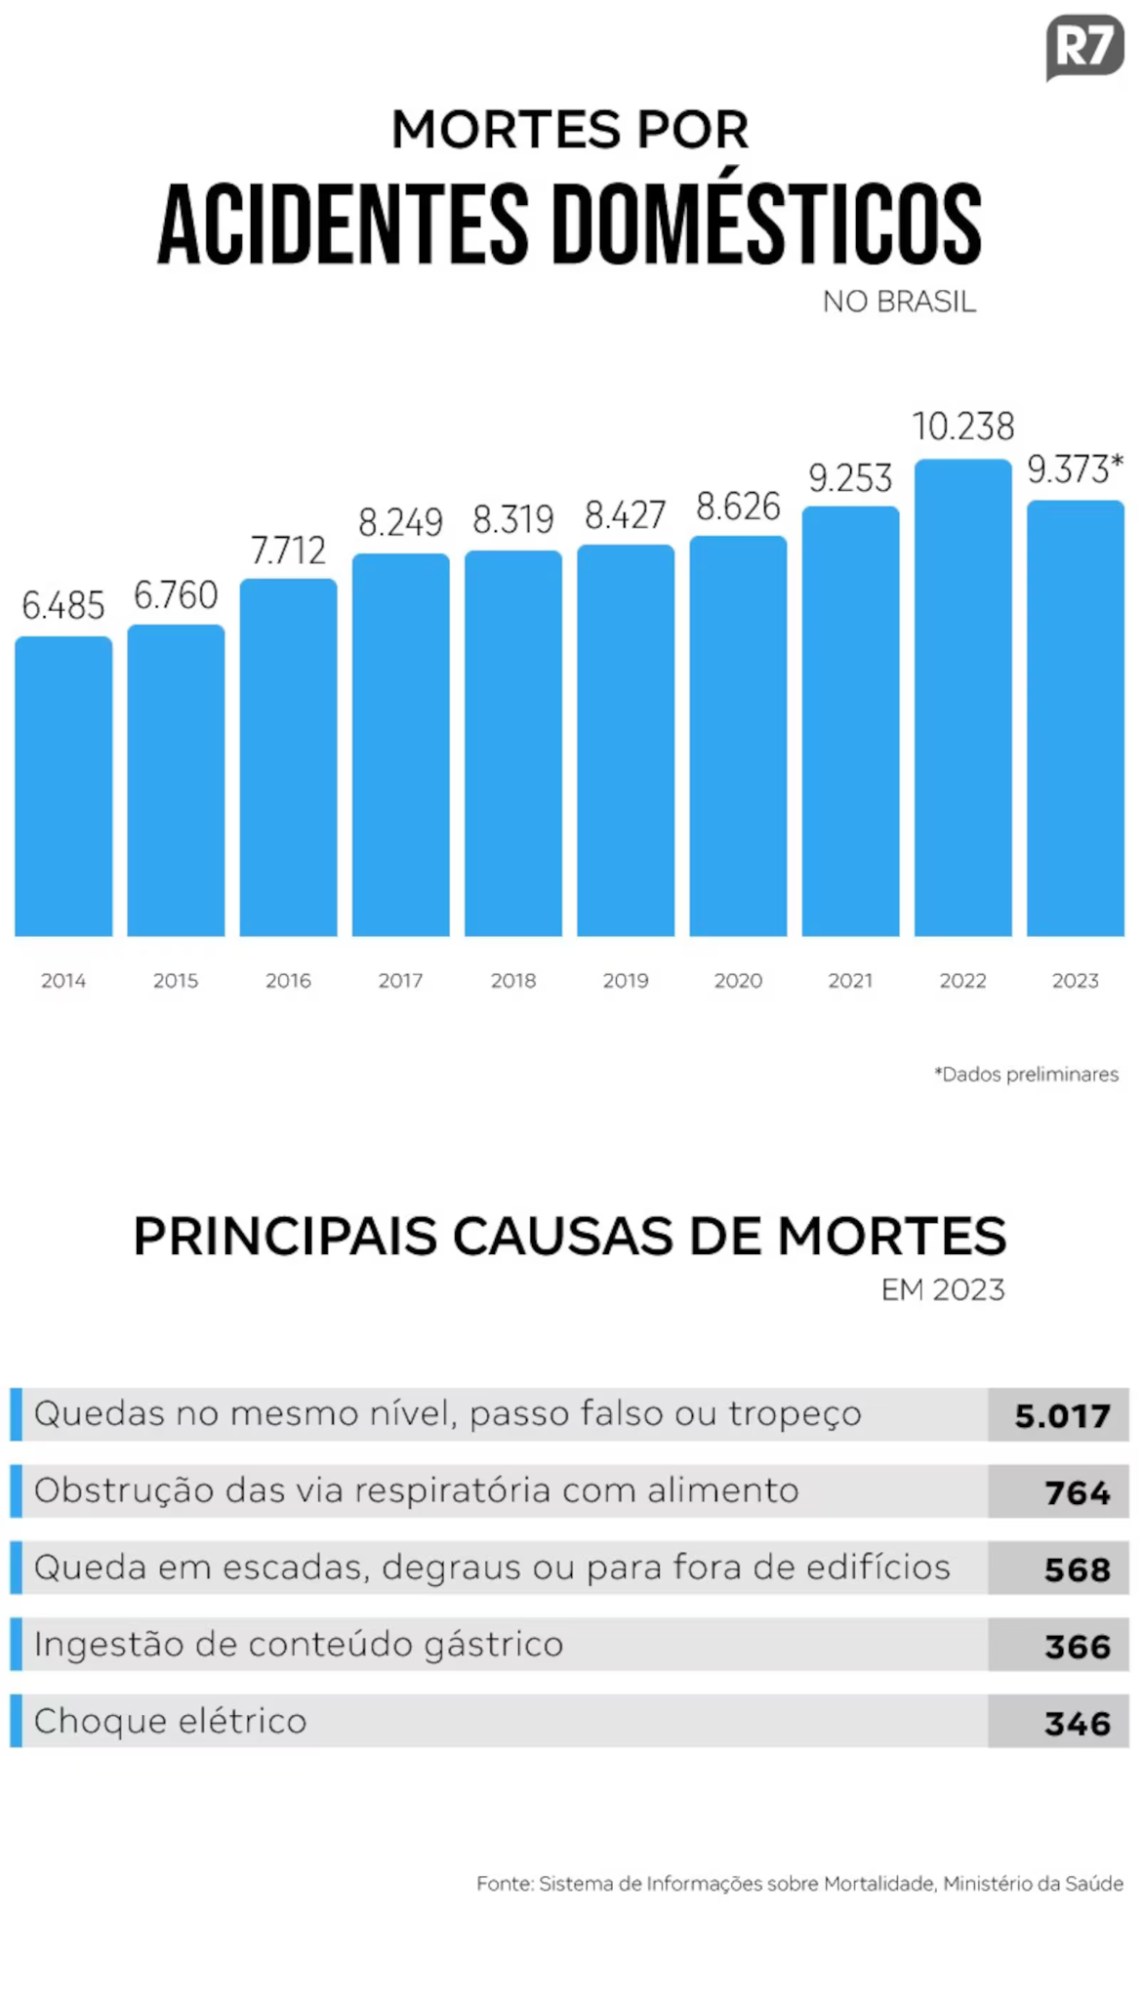
\includegraphics[scale=0.3]{imagens/acidentes_domesticos.png}
\end{center}
\legend{Fonte: Ministério da Saúde via R7 (2024).}
\end{figure}


\section{Análise da Concorrência}

Após análise de mercado, foram identificados os seguintes serviços disponíveis no mercado.

\subsection{Are You Dead?}

O \textit{Are You Dead?}, também conhecido por Demumu, é um aplicativo chinês de chamadas de emergência desenvolvido originalmente para jovens que moram sozinhos. O sistema exige que o usuário realize check-ins periódicos e, em caso de ausência prolongada, envia notificações para contatos de emergência previamente cadastrados.

\subsection{Ok Alone}

O \textit{Ok Alone} é um aplicativo canadense voltado principalmente para trabalhadores solitários e pessoas em situações de risco. O sistema oferece check-ins periódicos, monitoramento por inatividade prolongada, botão de emergência manual e geração de relatórios.

\subsection{Senior Safety App}

O \textit{Senior Safety App} é um aplicativo de segurança voltado para idosos. A solução oferece alertas automáticos para cuidadores, monitoramento de inatividade, detecção de quedas do dispositivo, geolocalização e sistema de chamadas em sequência para contatos de emergência.

\subsection{Comparativo}

O Quadro~\ref{quad} apresenta uma comparação entre as funcionalidades da solução proposta e dos sistemas concorrentes.

\begin{table}[H]
\caption{Comparação de funcionalidades entre Linha Vital e concorrentes}
\label{quad}
\centering

\begin{tabular}{p{6cm}cccc}
\hline
\textbf{Funcionalidade} &
\textbf{Linha Vital} &
\textbf{Demumu} &
\textbf{Ok Alone} &
\textbf{Senior Safety} \\

\hline

Check-in automático periódico & Sim & Sim & Sim & Sim \\
Monitoramento por inatividade & Sim & Sim & Sim & Sim \\
Acionamento automático de contatos & Sim & Sim & Sim & Sim \\
Múltiplos contatos por categoria & Sim & Não & Sim & Sim \\
Botão de emergência (SOS) & Sim & Não & Sim & Sim \\
Acionamento por botão físico & Sim & Não & Não & Não \\
Integração com órgãos públicos & Sim & Não & Sim & Não \\
Foco em uso doméstico/social & Sim & Sim & Não & Sim \\
Hardware único & Sim & Sim & Sim & Sim \\
Modelo sem central paga & Sim & Sim & Não & Sim \\

\hline
\end{tabular}

\fonte{Elaborado pelos autores.}

\end{table}